\documentclass[12pt]{article}
\usepackage[a4paper, margin=0.8in]{geometry}
\usepackage[utf8]{inputenc}
\usepackage[english]{babel}
\usepackage{amsmath}
\usepackage{appendix}
\usepackage{biblatex}
\usepackage{float}
\usepackage{graphicx}
\usepackage{listings}
\usepackage{titlesec}
\usepackage{xcolor}

\titlespacing{\subsection}{0pt}{12pt}{6pt}
\titleformat*{\subsection}{\small\bfseries}
\setlength\parindent{0pt}
\addbibresource{references.bib}

\definecolor{codegreen}{rgb}{0,0.6,0}
\definecolor{codegray}{rgb}{0.5,0.5,0.5}
\definecolor{codepurple}{rgb}{0.58,0,0.82}
\definecolor{backcolour}{rgb}{0.95,0.95,0.92}

\lstdefinestyle{code}{
    backgroundcolor=\color{backcolour},
    commentstyle=\color{codegreen},
    keywordstyle=\color{magenta},
    numberstyle=\tiny\color{codegray},
    stringstyle=\color{codepurple},
    basicstyle=\ttfamily\footnotesize,
    breaklines=true,
    showstringspaces=false,
}
\lstset{style=code}

\title{Reinforcement Learning Coursework 1}
\author{Yong Shen Tan}
\date{9 November 2020}

\begin{document}

\newpage
\begin{center}
    \vspace*{10em}
    \textsc{\huge Imperial College London}\vspace{2em}
    
    \textsc{\Large Department of Computing}\vspace{2em}
    
    \rule{\linewidth}{.2mm}\vspace{2em}
    \makeatletter
        {\huge \textbf \@title\par}\vspace{2em}
    \makeatother
    \rule{\linewidth}{.2mm}\vspace{2em}
    
    \large
    \textit{Author:}
    
    \medskip
    \makeatletter
        \@author
    \makeatother
    
    (CID 01055349)\vspace{2em}
    
    \today
\end{center}

\newpage
\section*{Question 1: Understanding of MDPs}

\textit{Relevant Python code for this question can be found in Appendix \ref{appendix:q1}}.

\subsection*{Part 1.a}

The sequences of states and rewards computed using the CID of \textbf{1055349} produces the following trace:
\begin{equation}
    \tau = s_3\ 1\ s_2\ 0\ s_3\ 1\ s_3\ 1\ s_1\ 3\ s_2\ 0\ s_3\ 1\
\end{equation}

\subsection*{Part 1.b}
From the observed trace above, we can construct the following MDP graph:

\begin{figure}[H]
    \centering
    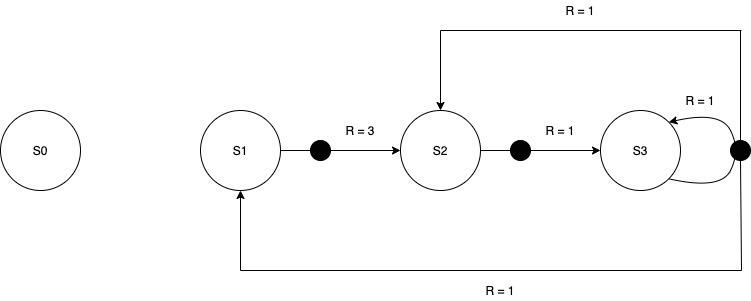
\includegraphics[width=0.7\textwidth]{figures/1b.png}
    \caption{Minimal MDP Graph from Observed Trace}
    \label{figure:1b}
\end{figure}

Following the trace, we can draw the transitions between states, where the action chosen is the deterministic one, \textit{``no choice"}, represented as a black circle. The trace also gives us the immediate rewards in that time step as we transition between states, indicated by the arrows. We do the same for all state transitions in the trace, eventually obtaining the MDP graph seen in Figure \ref{figure:1b}. In the case where the trace goes from one state to itself, such as \(s_3\) to \(s_3\) as seen in the trace, we draw a self-connecting transition.

\subsection*{Part 1.c (1)}
The transition probabilities are independent of the action we choose, allowing us to describe the transition matrix of the MDP as a 4x4 matrix, \(P_{ss'}\):\vspace{1em}

\begin{minipage}{.5\textwidth}
    \begin{equation}
    P_{ss'} = 
        \begin{pmatrix}
            p_{00} & p_{01} & p_{02} & p_{03}\\
            p_{10} & p_{11} & p_{12} & p_{13}\\
            p_{20} & p_{21} & p_{22} & p_{23}\\
            p_{30} & p_{31} & p_{32} & p_{33}
        \end{pmatrix}
    \end{equation}
\end{minipage}
\begin{minipage}{.5\textwidth}
    \begin{equation}
    P_{ss'} = 
        \begin{pmatrix}
            0 & 0 & 0 & 0\\
            0 & 0 & 1 & 0\\
            0 & 0 & 0 & 1\\
            0 & \frac{1}{3} & \frac{1}{3} & \frac{1}{3}
        \end{pmatrix}
    \end{equation}
\end{minipage}
\vspace{1em}

Based on the trace observed we can say for certain that the probability of transitioning between the states with arrows shown in Figure \ref{figure:1b} is more than 0. The other transition probabilities are unknown and cannot be determined as we have not observed those state transitions. That is to say:\vspace{1em}

\begin{minipage}{.5\textwidth}
    \noindent
    \begin{equation}
        p_{ss'} \in [p_{12},\ p_{12},\ p_{31},\ p_{32},\ p_{33}] > 0
    \end{equation}
\end{minipage}
\begin{minipage}{.5\textwidth}
    \noindent
    \begin{equation}
        p_{ss'} \not\in [p_{12},\ p_{12},\ p_{31},\ p_{32},\ p_{33}] \in [0,1]
    \end{equation}
\end{minipage}
\vspace{0.1em}

Assuming that our single trace fully describes the transition dynamics of the MDP, we obtain the following transition matrix, \(P_{ss'}\), shown in (3).

\subsection*{Part 1.c (2)}
The immediate rewards are independent of the action we choose, allowing us to describe the reward matrix of the MDP as a 4x4 matrix, \(R_{ss'}\):\vspace{1em}

\begin{minipage}{.5\textwidth}
    \begin{equation}
    R_{ss'} = 
        \begin{pmatrix}
            k_{00} & k_{01} & k_{02} & k_{03}\\
            k_{10} & k_{11} & k_{12} & k_{13}\\
            k_{20} & k_{21} & k_{22} & k_{23}\\
            k_{30} & k_{31} & k_{32} & k_{33}
        \end{pmatrix}
    \end{equation}
\end{minipage}
\begin{minipage}{.5\textwidth}
    \begin{equation}
    R_{ss'} = 
        \begin{pmatrix}
            0 & 0 & 0 & 0\\
            0 & 0 & 3 & 0\\
            0 & 0 & 0 & 1\\
            0 & 1 & 1 & 1
        \end{pmatrix}
    \end{equation}
\end{minipage}
\vspace{1em}

Based on the trace observed we can say for certain that the immediate reward collected when transitioning between the states with arrows shown in Figure \ref{figure:1b} is more than 0. The other immediate rewards are unknown and cannot be determined as we have not observed those state transitions. That is to say:\vspace{1em}

\begin{minipage}{.5\textwidth}
    \noindent
    \begin{equation}
        k_{ss'} \in [k_{12},\ k_{12},\ k_{31},\ k_{32},\ k_{33}] > 0
    \end{equation}
\end{minipage}
\begin{minipage}{.5\textwidth}
    \noindent
    \begin{equation}
        k_{ss'} \not\in [k_{12},\ k_{12},\ k_{31},\ k_{32},\ k_{33}] \rightarrow unknown
    \end{equation}
\end{minipage}
\vspace{0.1em}

Assuming that our single trace fully describes the reward dynamics of the MDP, we obtain the following reward matrix, \(R_{ss'}\), shown in (7).

\subsection*{Part 1.c (3)}
Given that we only have a single trace of the MDP, which might also be an incomplete episode, we are not able to use Monte-Carlo methods. We also do not have information about the transition or reward matrix of the MDP and are thus not able to use Dynamic Programming methods. This leaves us with Temporal Difference methods for estimating the value of \(s_3\).

\begin{equation}
V(s_t) \leftarrow V(s_t) + \alpha (r_{t+1} + \gamma V(s_{t+1}) - V(s_t))
\end{equation}

Applying the TD(0) algorithm on the observed trace of states and rewards, where we do iterative updates of our estimated value functions based on (10), we are able to compute \(V(s_3) = 1\). A learning rate, \(\alpha\), of 1 was used given that we only have a single trace. The discount factor, \(\gamma\), was set to 1 to obtain the undiscounted value of \(s_3\).\medskip

\section*{Question 2: Understanding of Grid Worlds}

\textit{Relevant Python code for this question can be found in Appendix \ref{appendix:q2}}.

\subsection*{Part 2.a}

Using the last 3 digits of the CID of \textbf{1055349}, we obtain the following:

\begin{minipage}{.3\textwidth}
    \begin{equation}
        s_{reward} = s_2
    \end{equation}      
\end{minipage}
\begin{minipage}{.3\textwidth}
    \begin{equation}
        p = 0.45
    \end{equation}
\end{minipage}
\begin{minipage}{.3\textwidth}
    \begin{equation}
        \gamma = 0.4
    \end{equation}
\end{minipage}

\subsection*{Part 2.b (1-3)}

The optimal value function and policy were computed using the Dynamic Programming value iteration algorithm, shown in Figures \ref{figure:2b2} and \ref{figure:2b3} respectively, with the stopping condition \(\theta = 0.00001\). When determining the optimal policy for a given state in the case where there are multiple equally optimal actions, we assume we randomly pick one from those actions with equal probabilities.

\begin{figure}[H]
  \centering
  \begin{minipage}[b]{0.3\textwidth}
    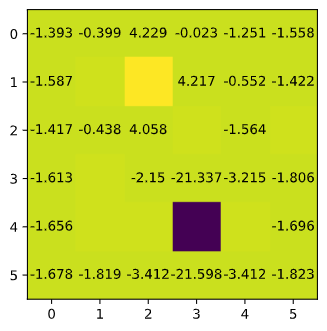
\includegraphics[width=\textwidth]{figures/2b2.png}
    \caption{DP Optimal Value Function}
    \label{figure:2b2}
  \end{minipage}
  \hspace{3em}
  \begin{minipage}[b]{0.3\textwidth}
    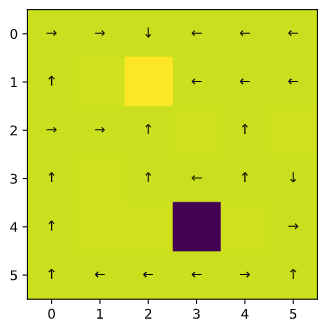
\includegraphics[width=\textwidth]{figures/2b3.png}
    \caption{DP Optimal Policy}
    \label{figure:2b3}
  \end{minipage}
\end{figure}

\subsection*{Part 2.b (4)}

If we define the ideal policy as one that leads to the reward state in the least numbers of moves, increasing \(p\) improves the optimal policy towards the ideal policy; a higher \(p\) indicates there's less stochasticity in our agent's actions, allowing it to better estimate the value of states and hence a better policy. This was verified by testing with \(p\) values of 0.1, 0.25 and 0.9.\medskip

Increasing \(\gamma\) causes value iteration to converge more slowly to the optimal value function. A higher \(\gamma\) implies less discounting of rewards as the agent is more far-sighted, causing the difference of the estimated value function between iterations to be larger and thus requiring more iterations for the difference to fall below \(\delta\). This was verified by testing with \(\gamma\) values of 0.25 and 0.75.

\subsection*{Part 2.c (1-2)}

The optimal value function and policy were computed using the Monte Carlo iterative optimisation algorithm, shown in Figures \ref{figure:2c2_value} and \ref{figure:2c2_policy} respectively. The agent was trained over 1000 episodes using an \(\epsilon\)-greedy policy, with \(\epsilon = 0.1\), and a learning rate \(\alpha = 0.05\). We assume that our agent would have explored each state at least \(\frac{1}{\alpha}\) times, such that scaling by \(\alpha\) is an accurate estimate of its value.

\begin{figure}[H]
  \centering
  \begin{minipage}[b]{0.3\textwidth}
    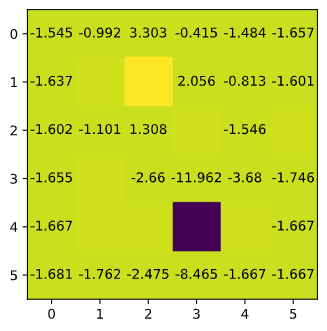
\includegraphics[width=\textwidth]{figures/2c2_value.png}
    \caption{MC Estimate of Optimal Value Function}
    \label{figure:2c2_value}
  \end{minipage}
  \hspace{3em}
  \begin{minipage}[b]{0.3\textwidth}
    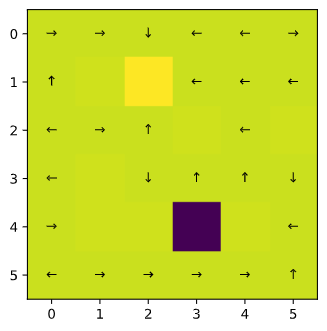
\includegraphics[width=\textwidth]{figures/2c2_policy.png}
    \caption{MC Estimate of Optimal Policy}
    \label{figure:2c2_policy}
  \end{minipage}
\end{figure}

\subsection*{Part 2.c (3)}

The learning curve in Figure \ref{figure:2c3}, derived using MC, was averaged over 1000 repetitions of 1000 episodes. 1000 repetitions was chosen as it sufficiently reduced noise between repetitions such that we can more clearly see the agent learning over episodes and the rewards reach a plateau.

\begin{figure}[H]
    \centering
    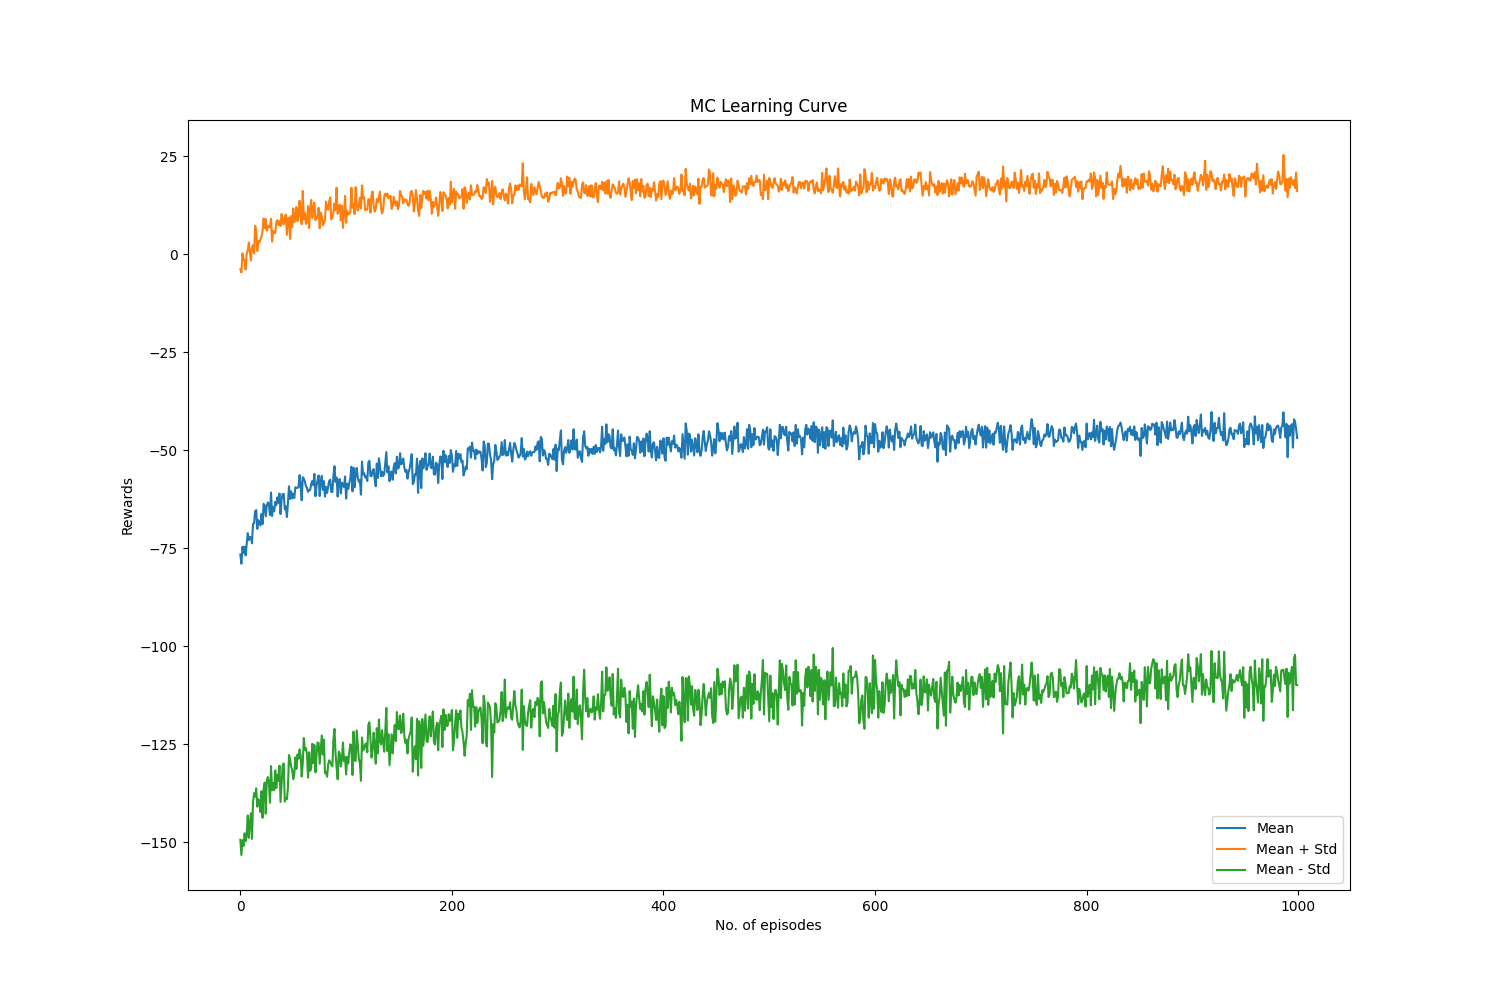
\includegraphics[width=0.7\textwidth]{figures/2c3.png}
    \caption{Learning Curve of MC Agent}
    \label{figure:2c3}
\end{figure}

\subsection*{Part 2.c (4)}

Figure \ref{figure:2c4_alpha} shows that increasing \(\alpha\) causes the agent to learn more quickly but plateau earlier. As the environment is stationary, giving more weight to recent episodes as our agent learns pulls the estimated value function faster to the optimal one. A lower \(\alpha\) however, leads to more steady learning and higher eventual rewards, as more information is used to inform its policy.

\begin{figure}[H]
    \centering
    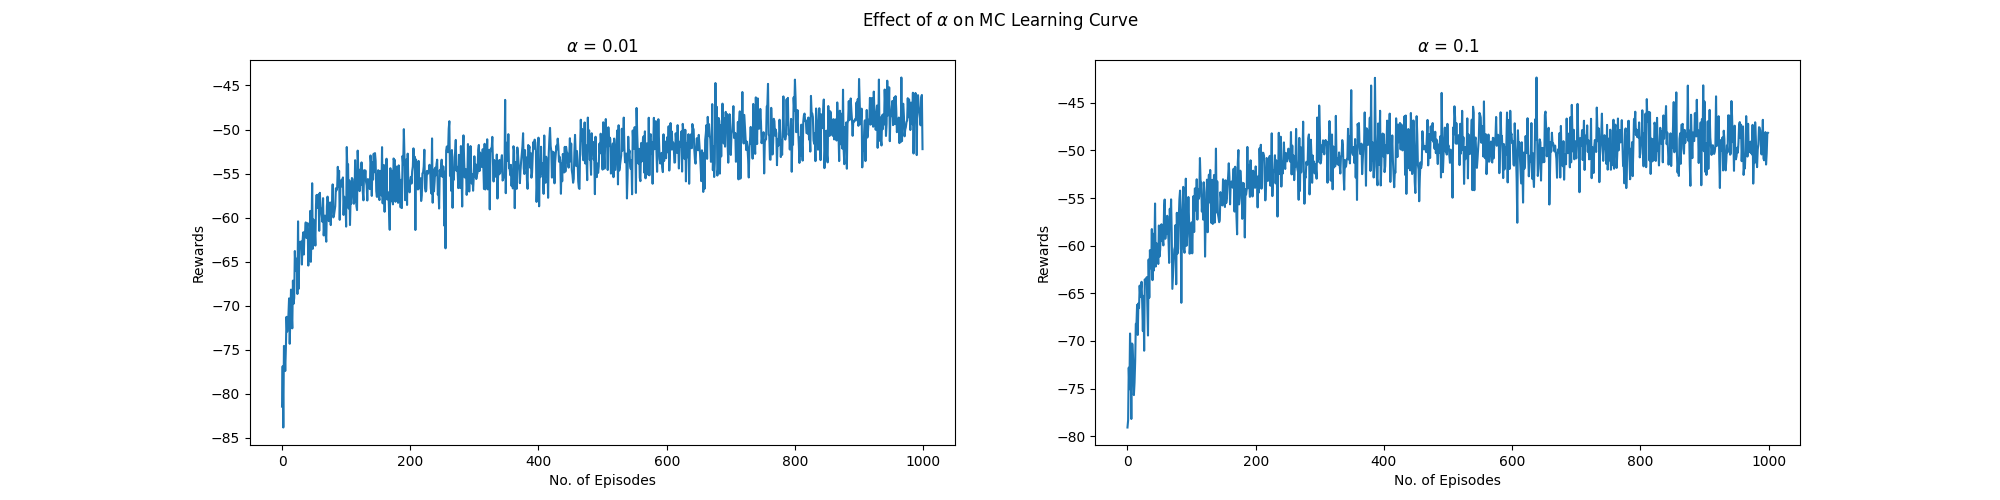
\includegraphics[width=\textwidth]{figures/2c4_alpha.png}
    \caption{Learning Curve of MC Agent (Varying \(\alpha\))}
    \label{figure:2c4_alpha}
\end{figure}

Figure \ref{figure:2c4_epsilon} shows that increasing \(\epsilon\) causes slightly greater variance in the learning curve. This makes sense as our agent might encounter poor rewards while exploring the grid world more as it's not following the optimal policy.

\begin{figure}[H]
    \centering
    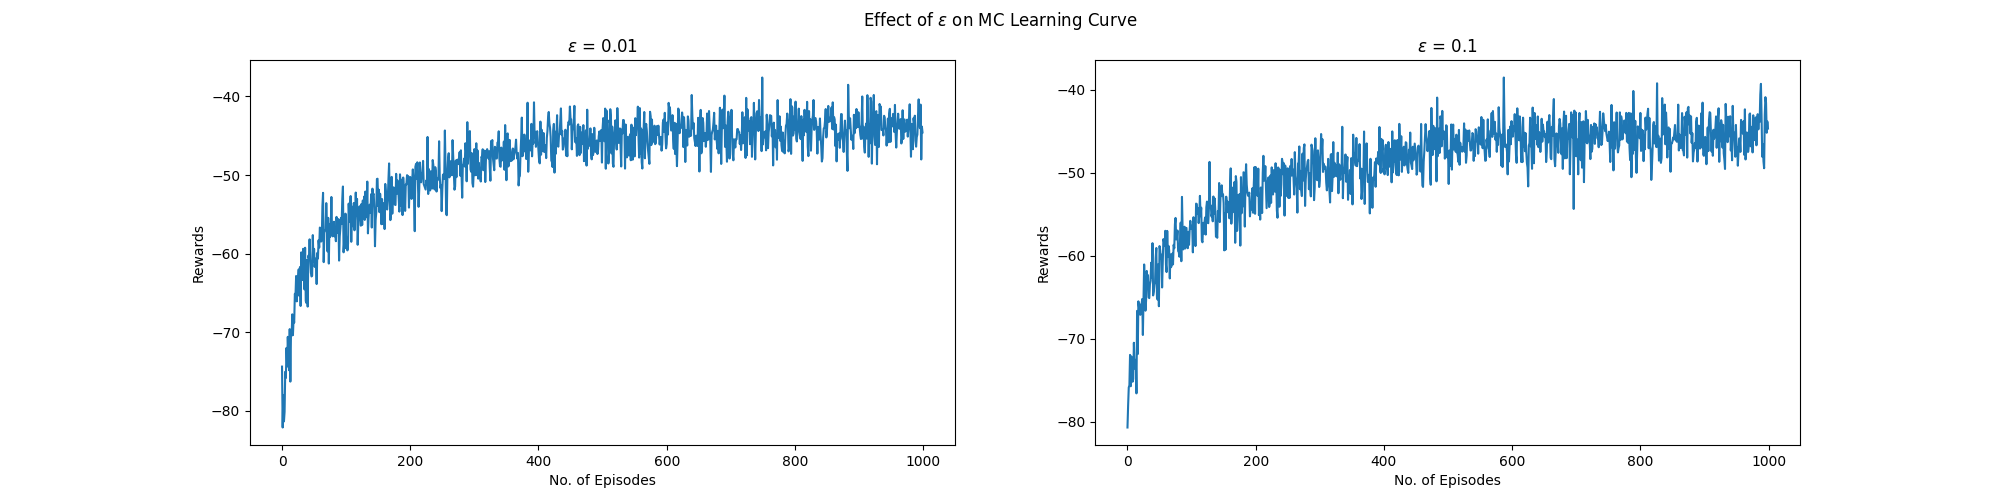
\includegraphics[width=\textwidth]{figures/2c4_epsilon.png}
    \caption{Learning Curve of MC Agent (Varying \(\epsilon\))}
    \label{figure:2c4_epsilon}
\end{figure}

\subsection*{Part 2.d (1-2)}

The optimal value function and policy were computed using the Q-Learning algorithm, shown in Figures \ref{figure:2d2_value} and \ref{figure:2d2_policy} respectively. The agent was trained over 1000 episodes using an \(\epsilon\)-greedy policy, with \(\epsilon = 0.1\), and a learning rate \(\alpha = 0.05\). We assume that our agent would have explored each state at least \(\frac{1}{\alpha}\) times, such that scaling by \(\alpha\) is an accurate estimate of its value.

\begin{figure}[H]
  \centering
  \begin{minipage}[b]{0.3\textwidth}
    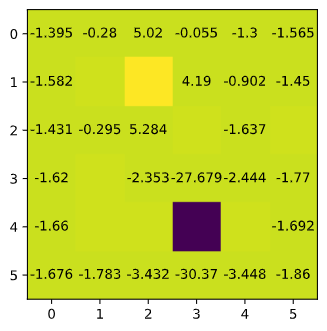
\includegraphics[width=\textwidth]{figures/2d2_value.png}
    \caption{TD Estimate of Optimal Value Function}
    \label{figure:2d2_value}
  \end{minipage}
  \hspace{3em}
  \begin{minipage}[b]{0.3\textwidth}
    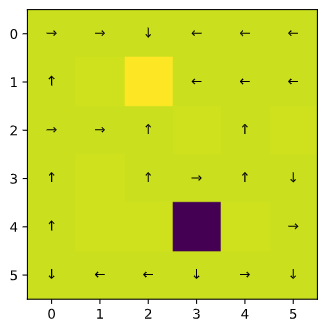
\includegraphics[width=\textwidth]{figures/2d2_policy.png}
    \caption{TD Estimate of Optimal Policy}
    \label{figure:2d2_policy}
  \end{minipage}
\end{figure}

\subsection*{Part 2.d (3)}

The learning curve in Figure \ref{figure:2d3}, derived using TD, was averaged over 1000 repetitions of 1000 episodes. 1000 repetitions was chosen as it sufficiently reduced noise between repetitions such that we can more clearly see the agent learning over episodes and the rewards reach a plateau.

\begin{figure}[H]
    \centering
    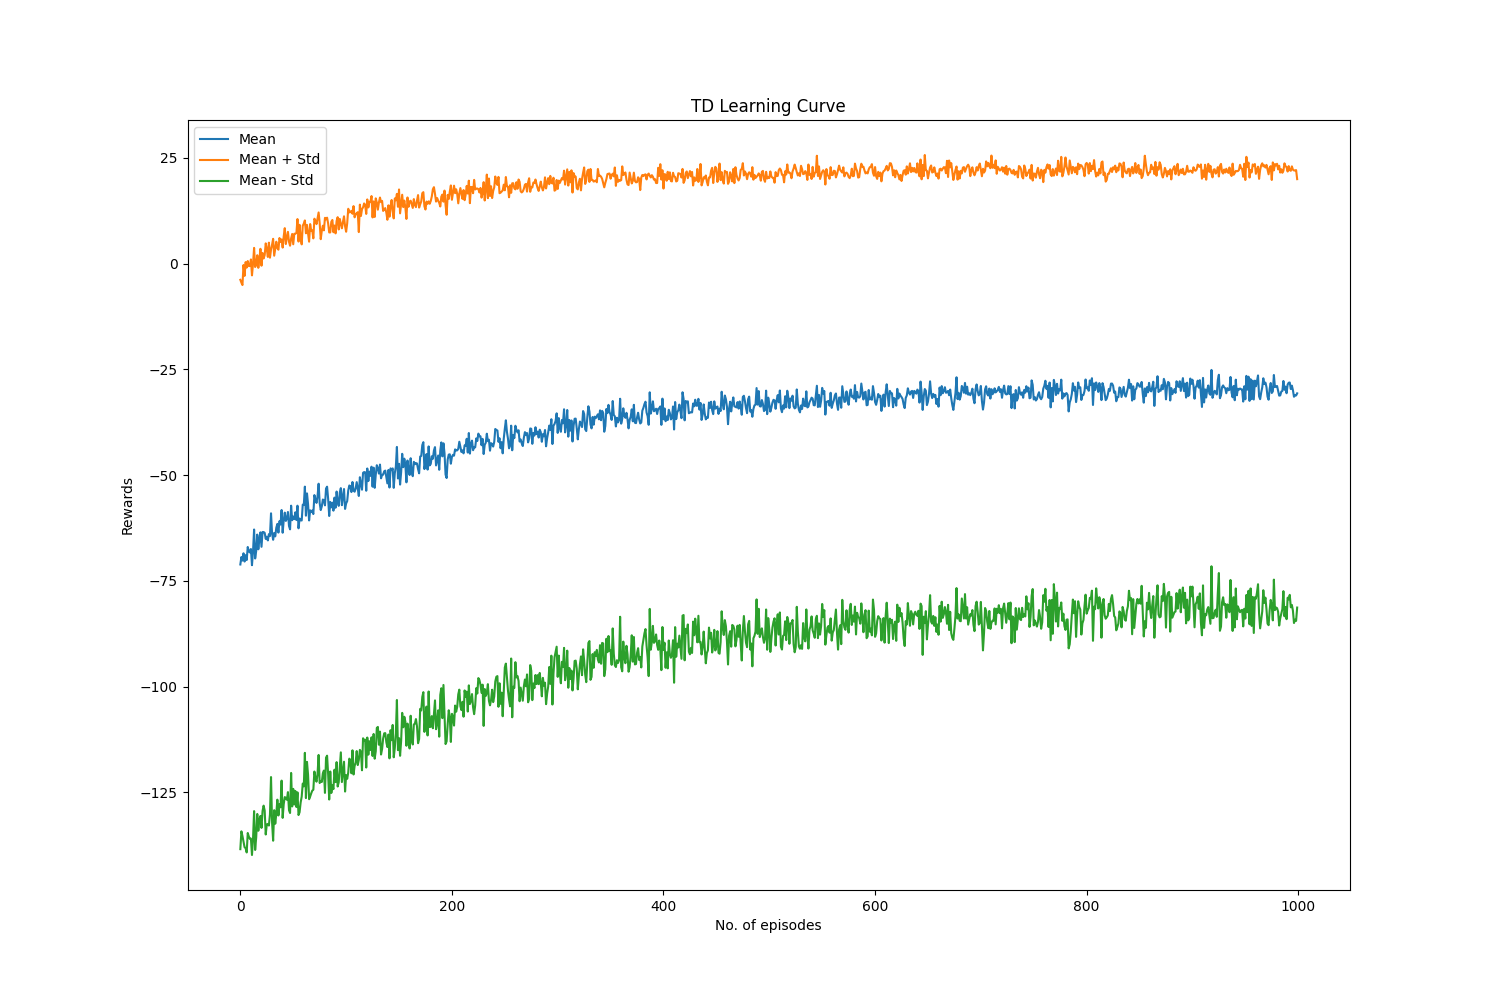
\includegraphics[width=0.7\textwidth]{figures/2d3.png}
    \caption{Learning Curve of TD Agent}
    \label{figure:2d3}
\end{figure}

\subsection*{Part 2.d (4)}

Figure \ref{figure:2d4_alpha} shows that increasing \(\alpha\) causes the agent to learn more quickly but plateau earlier. As the environment is stationary, giving more weight to recent episodes as our agent learns pulls the estimated value function faster to the optimal one.

\begin{figure}[H]
    \centering
    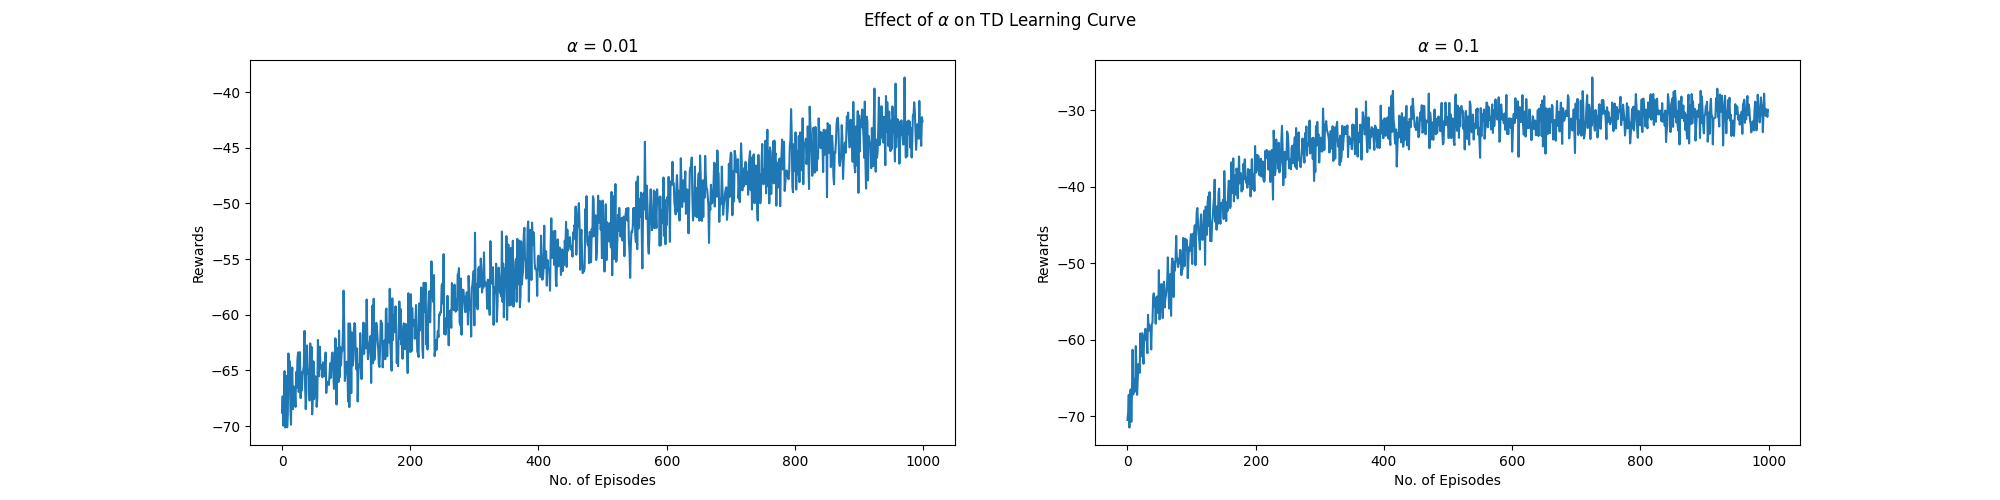
\includegraphics[width=\textwidth]{figures/2d4_alpha.png}
    \caption{Learning Curve of TD Agent (Varying \(\alpha\))}
    \label{figure:2d4_alpha}
\end{figure}

Figure \ref{figure:2d4_epsilon} shows that increasing \(\epsilon\) causes slightly greater variance in the learning curve. This makes sense as our agent might encounter poor rewards while exploring the grid world more as it's not following the optimal policy.

\begin{figure}[H]
    \centering
    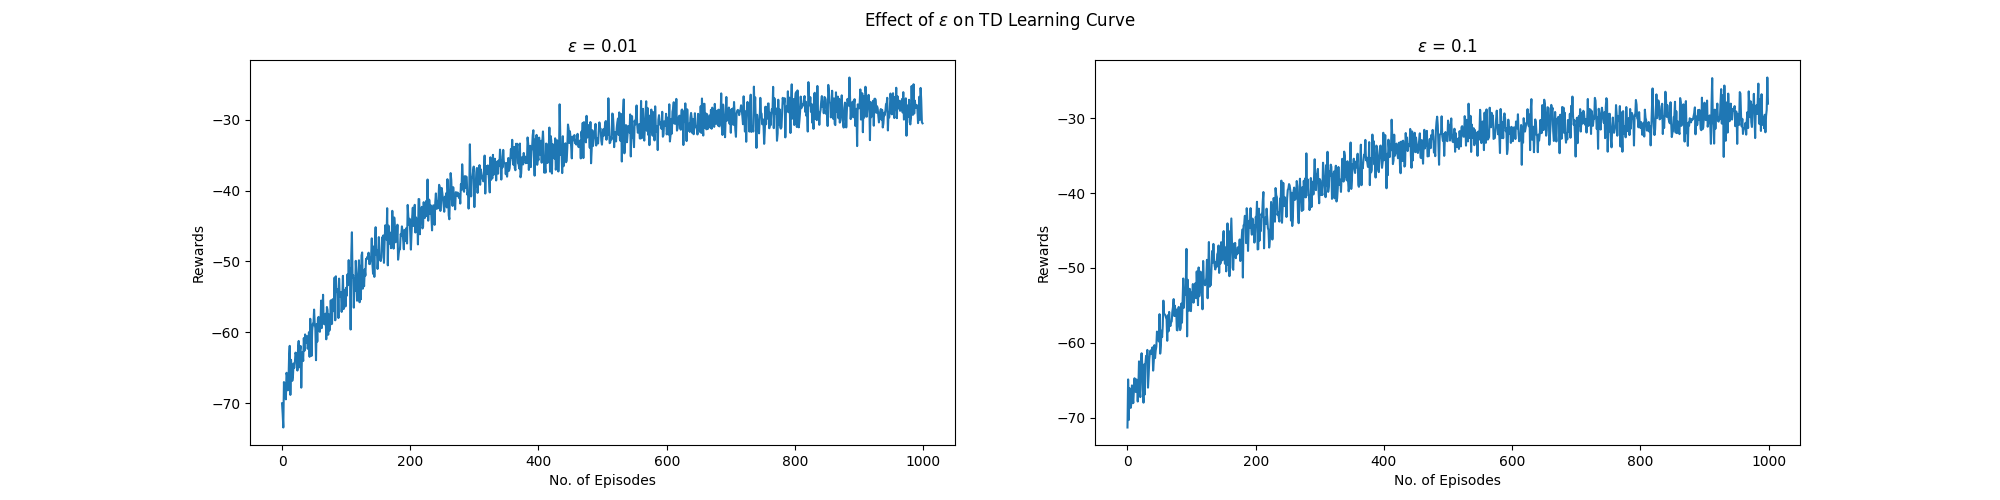
\includegraphics[width=\textwidth]{figures/2d4_epsilon.png}
    \caption{Learning Curve of TD Agent (Varying \(\epsilon\))}
    \label{figure:2d4_epsilon}
\end{figure}

\subsection*{Part 2.e (1)}

It is observed from Figure \ref{figure:2e1} that the TD method learns more quickly when estimating the optimal value function compared to the MC implementation, seen from the steeper slope. This agrees with the theory that TD methods are usually more efficient than MC methods at learning, as MC uses complete returns to improve estimates while TD immediately uses estimates of successor states.\medskip

Theoretically, MC methods should be more accurate compared to TD methods as they are less prone to bias. However, as we are randomly initialising our starting state each episode, this disadvantage of TD methods is reduced and it performs more accurately as seen from the lower estimation error compared to MC methods.

\begin{figure}[H]
  \centering
  \begin{minipage}[b]{0.4\textwidth}
    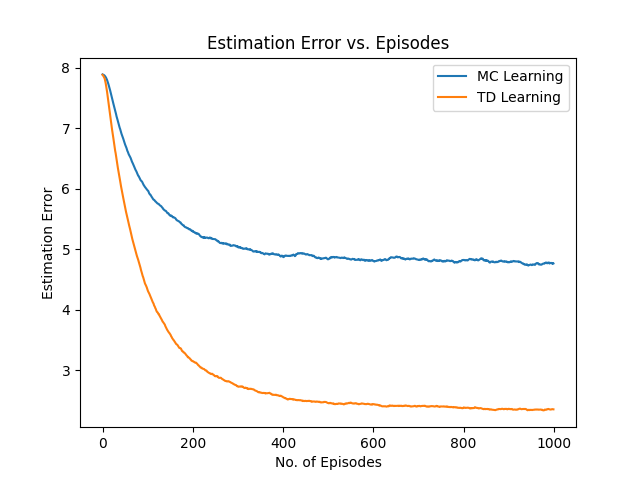
\includegraphics[width=\textwidth]{figures/2e1.png}
    \caption{Estimation Error vs. Episodes}
    \label{figure:2e1}
  \end{minipage}
  \hspace{3em}
  \begin{minipage}[b]{0.4\textwidth}
    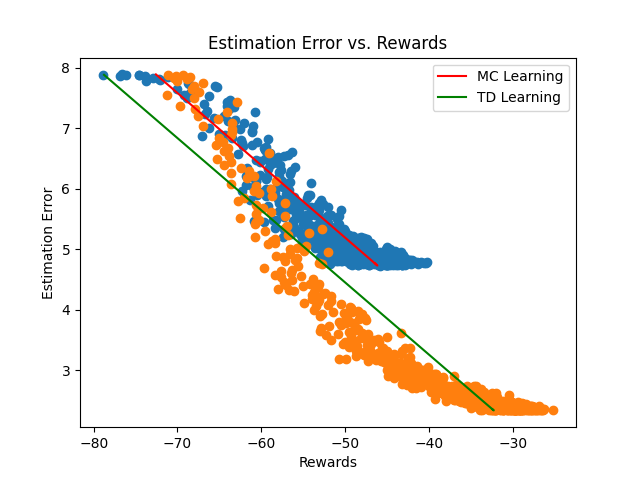
\includegraphics[width=\textwidth]{figures/2e2.png}
    \caption{Estimation Error vs. Rewards}
    \label{figure:2e2}
  \end{minipage}
\end{figure}

\subsection*{Part 2.e (2)}

Figure \ref{figure:2e2} characterises how the rewards collected by the MC (blue) and TD (orange) agents during each episode depends on how accurately it estimated the optimal value function. The variability in the data accounts for the exploration done by our agents as well as the stochasticity of the environment.\medskip

The plots for both show a clear trend that as the estimation error decreases, our rewards improve as our agent is able to reap more rewards by choosing the most optimal action in each state that maximises its value. This highlights that it is highly important to have a good estimation of the optimal value function to gain higher rewards. However, a good estimate doesn't necessarily guarantee high rewards as there is high stochasticity in the environment, due to \(p = 0.4\), that the agent cannot plan for.

\subsection*{Part 2.e (3)}

As seen from Figure \ref{figure:2e1}, the TD method outperforms the MC one at learning the optimal policy. Furthermore, in this case where exploring starts were used, the inherent bias of TD learning can be reduced such that it performs more accurately compared to MC learning. Figures \ref{figure:2e3_alpha} and \ref{figure:2e3_epsilon} show that varying the learning parameters, \(\epsilon\) and \(\alpha\), do not really change the performance of MC over TD.\medskip

However, as the grid world is a Markovian environment and TD methods exploit the Markov property, they tend to perform better in the given environment. It's possible for MC methods to outperform TD methods in a non-Markovian environment as MC is not dependent on the Markov property and instead uses empirical experiences.\medskip

\begin{figure}[H]
  \centering
  \begin{minipage}[b]{0.45\textwidth}
    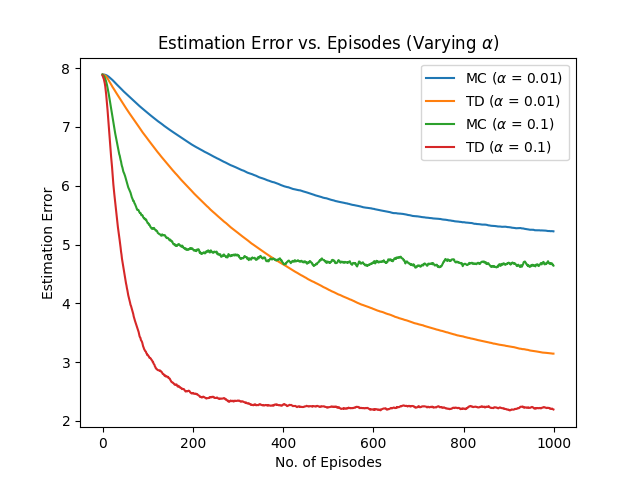
\includegraphics[width=\textwidth]{figures/2e3_alpha.png}
    \caption{Estimation Error vs. Episodes With Varying \(\alpha\)}
    \label{figure:2e3_alpha}
  \end{minipage}
  \hspace{3em}
  \begin{minipage}[b]{0.45\textwidth}
    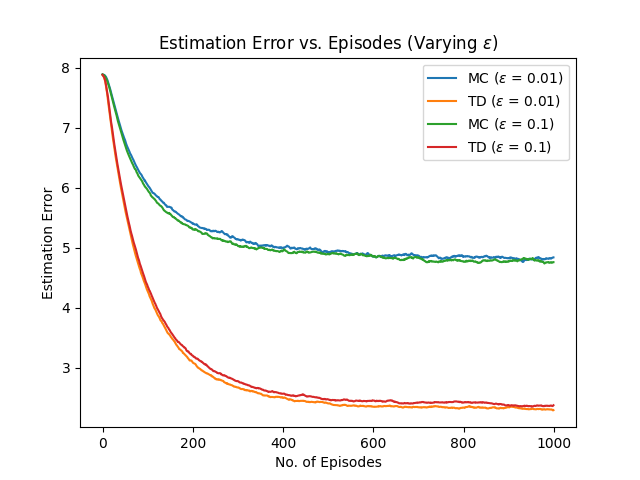
\includegraphics[width=\textwidth]{figures/2e3_epsilon.png}
    \caption{Estimation Error vs. Episodes With Varying \(\epsilon\)}
    \label{figure:2e3_epsilon}
  \end{minipage}
\end{figure}

\newpage

\newpage
\appendixpage
\appendix
\section{Python Code for Question 1}
\label{appendix:q1}
\lstinputlisting[language=Python]{./code/Q1.py}
\section{Python Code for Question 2}
\lstinputlisting[language=Python]{./code/Q2.py}
\label{appendix:q2}

\end{document}